%
%===============>>  ПРОБНИК 1 <<=============
%

%BEGIN_FOLD % ====>>_____ Вариант 1 _____<<====
\begin{training}[1]
	\title{Часть 1}
	\egepreambone
	\begin{listofex}
		%1
		\item
		\begin{minipage}[t]{\bodywidth}
			В треугольнике \( ABC \) угол \( C \) равен \( 110\degree \), \( AD \) и \( BE \) --- биссектрисы, пересекающиеся в точке \( O \). Найдите угол \( AOB \). Ответ дайте в градусах.
			\foranswer
		\end{minipage}
		\gapwidth
		\begin{minipage}[t]{\picwidth}
			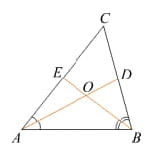
\includegraphics[align=t, width=\linewidth]{\picpath/prob_2_1}
		\end{minipage}
		%2
		\item
		\begin{minipage}[t]{\bodywidth}
			Прямоугольный параллелепипед описан около цилиндра, радиус основания и высота которого равны \( 2 \). Найдите объём параллелепипеда.
			\foranswer
		\end{minipage}
		\gapwidth
		\begin{minipage}[t]{\picwidth}
			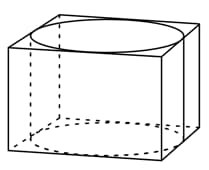
\includegraphics[align=t, width=\linewidth]{\picpath/prob_2_2}
		\end{minipage}
		%3
		\item На олимпиаде по русскому языку \( 400 \) участников разместили в трёх аудиториях. В первых двух удалось разместить по \( 110 \) человек, оставшихся перевели в запасную аудиторию в другом корпусе. Найдите вероятность того, что случайно выбранный участник писал олимпиаду в запасной аудитории.
		\foranswer
		%4
		\item На экзамене по геометрии школьник отвечает на один вопрос из списка экзаменационных вопросов. Вероятность того, что это вопрос по теме «Вписанная окружность», равна \( 0,15 \). Вероятность того, что это вопрос по теме «Тригонометрия», равна \( 0,3 \). Вопросов, которые одновременно относятся к этим двум темам, нет. Найдите вероятность того, что на экзамене школьнику достанется вопрос по одной из этих двух тем.
		\foranswer
	\end{listofex}
	\newpage
	\phantom{Часть 1}
	\begin{listofex}[resume]
		%5
		\item Найдите корень уравнения \( \log_9(x+6)=\log_9(4x-9) \)
		\foranswer
		%6
		\item Найдите значение выражения \( \dfrac{60n^{\tfrac{1}{18}}}{n^{\tfrac{1}{27}}\cdot n^{\tfrac{1}{54}}} \)
		\foranswer
		%7
		\item
		На рисунке изображён график функции \( y=f(x) \) и касательная к нему в точке с абсциссой \( x_0 \). Найдите значение производной функции \( f(x) \) в точке \( x_0 \).
		\begin{center}
			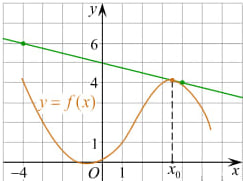
\includegraphics[align=t, width=0.4\linewidth]{\picpath/prob_2_4}
		\end{center}
		\foranswer
		%8
		\item К источнику с ЭДС \( \epsilon=55 \) В и внутренним сопротивлением \( r=0,5 \) Ом, хотят подключить нагрузку с сопротивлением \( R \) Ом. Напряжение на этой нагрузке, выражаемое в вольтах, даeтся формулой \( U=\dfrac{\epsilon R}{R+r} \).  При каком наименьшем значении сопротивления нагрузки напряжение на ней будет не менее \( 50 \) В? Ответ выразите в омах.
		\foranswer
		%9
		\item Теплоход проходит по течению реки до пункта назначения \( 247 \) км и после стоянки возвращается в пункт отправления. Найдите скорость течения, если скорость теплохода в неподвижной воде равна \( 16 \) км/ч, стоянка длится \( 7 \) часов, а в пункт отправления теплоход возвращается через \( 39 \) часов после отплытия из него. Ответ дайте в км/ч.
		\foranswer
		\newpage
		\hphantom{Часть 1}
		%10
		\item 
		На рисунке изображён график функции вида \( f(x)=ax^2+bx+c \), где числа \( a \), \( b \) и \( c \) --- целые. Найдите значение \( f(0,5) \).
		\begin{center}
			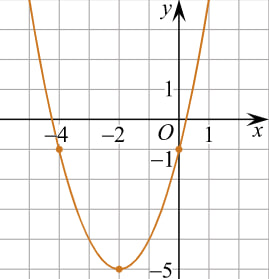
\includegraphics[align=t, width=0.4\linewidth]{\picpath/prob_2_5}
		\end{center}
		\foranswer
		%11
		\item Найдите наименьшее значение функции \( y=(x+3)^2(x+5)-1 \) на отрезке \( [-4;-1] \).
		\foranswer
		\egepreambtwo
		\title{Часть 2}
		%12
		\item a) Решите уравнение \( \cos2x+0,5=\cos^2x \). \\
		б) Найдите все корни этого уравнения, принадлежащие отрезку \( \left[ -2\pi;-\dfrac{\pi}{2} \right]  \)
		\newpage
		\hphantom{Часть 1}
		\item В основании прямой призмы \( ABCDA_1B_1C_1D_1 \) лежит квадрат \( ABCD \) со стороной \( 2 \), а высота призмы равна \( 1 \). Точка \( E \) лежит на диагонали \( BD_1 \), причём \( BE=1 \).\\
		а)  Постройте сечение призмы плоскостью \( A_1C_1E \).\\		
		б)  Найдите угол между плоскостью сечения и плоскостью \( ABC \).
		%14
		\item Решите неравенство: \( 5\cdot2^{2x+1}-21\cdot2^{x-1}\le0 \)
		%15
		\item Светлана Михайловна взяла кредит в банке на \( 4 \) года на сумму \( 4\: 420\: 000 \) рублей. Условия возврата кредита таковы: в конце каждого года банк увеличивает текущую сумму долга на \( 10\% \). Светлана Михайловна хочет выплатить весь долг двумя равными платежами --- в конце второго и четвертого годов. При этом платежи в каждом случае выплачиваются после начисления процентов. Сколько рублей составит каждый из этих платежей?
		%16
		\item В остроугольном треугольнике \( KMN \) проведены высоты \( KB \) и \( NA \).\\
		а)  Докажите, что угол \( ABK \) равен углу \( ANK \).	\\
		б)  Найдите радиус окружности, описанной около треугольника \( ABM \), если известно, что \( KN=8\sqrt{2} \) и \( \angle KMN=45\degree \).
		%17
		\item Найдите все \( a \), при каждом из которых уравнение 
		\[ \sqrt{2x+ax+2a+10}=x-1 \]
		не имеет действительных корней.
		%18
		\item Целые числа от \( 1 \) до \( n \) записаны в строчку. Под ними записаны те же числа в другом порядке. Может ли случиться так, что сумма каждого числа и записанного под ним есть точный квадрат.\\
		а)  при \( n=9 \),\\		
		б)  при \( n=11 \),\\		
		в)  при \( n=1996 \).
	\end{listofex}
\end{training}
%END_FOLD

%BEGIN_FOLD % ====>>_____ Вариант 2 _____<<====
\begin{training}[2]
	\title{Часть 1}
	\egepreambone
	\begin{listofex}
		%1
		\item
		Найдите площадь ромба, если его высота равна \( 2 \), а острый угол \( 30\degree \).
		\foranswer
		%2
		\item
		\begin{minipage}[t]{\bodywidth}
			Через среднюю линию основания треугольной призмы проведена плоскость, параллельная боковому ребру. Площадь боковой поверхности отсеченной треугольной призмы равна \( 8 \). Найдите площадь боковой поверхности исходной призмы.
			\foranswer
		\end{minipage}
		\gapwidth
		\begin{minipage}[t]{\picwidth}
			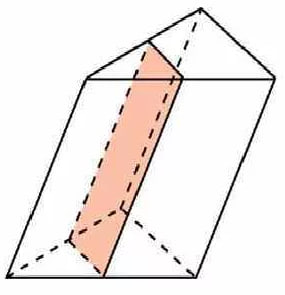
\includegraphics[align=t, width=\linewidth]{\picpath/prob_2_3}
		\end{minipage}
		%3
		\item В классе \( 16 \) учащихся, среди них два друга --- Олег и Вадим. Класс случайным образом разбивают на \( 4 \) равные группы. Найдите вероятность того, что Олег и Вадим окажутся в одной группе.
		\foranswer
		%4
		\item Вероятность того, что батарейка бракованная, равна \( 0,03 \). Покупатель в магазине выбирает случайную упаковку, в которой две таких батарейки. Найдите вероятность того, что обе батарейки окажутся исправными.
		\foranswer
		%5
		\item Найдите корень уравнения \( \cos\dfrac{\pi(4x+1)}{6}=\dfrac{\sqrt{3}}{2} \). В ответе запишите наибольший отрицательный корень.
		\foranswer
		\newpage
		\hphantom{Часть 1}
		%6
		\item Найдите \( -2\sin\left( \dfrac{\pi}{2}+\alpha \right) \), если \( \sin\alpha=-0,96 \) и \( \alpha\in(7\pi;8,5\pi) \).
		\foranswer
		%7
		\item 
		Материальная точка движется прямолинейно по закону \( x(t)=\dfrac{1}{6}t^2+5t+28 \) (где \( x \)  --- расстояние от точки отсчета в метрах, \( t \) --- время в секундах, измеренное с начала движения). В какой момент времени (в секундах) ее скорость была равна \( 6 \) м/с?
		\foranswer
		%8
		\item В ходе распада радиоактивного изотопа его масса уменьшается по закону \( m(t)=m_0\cdot2^{-t/T} \), где \( m_0 \) --- начальная масса изотопа, \( t \) --- время, прошедшее от начального момента, \( T \) --- период полураспада. В начальный момент времени масса изотопа \( 188 \) мг. Период его полураспада составляет \( 3 \) мин. Найдите, через сколько минут масса изотопа будет равна \( 47 \) мг.
		\foranswer
		%9
		\item Имеется два сосуда. Первый содержит \( 100 \) кг, а второй --- \( 20 \) кг раствора кислоты различной концентрации. Если эти растворы смешать, то получится раствор, содержащий \( 72\% \) кислоты. Если же смешать равные массы этих растворов, то получится раствор, содержащий \( 78\% \) кислоты. Сколько килограммов кислоты содержится в первом сосуде?
		\foranswer
		\newpage
		\hphantom{Часть 1}
		%10
		\item 
		На рисунке изображён график функции \( f(x)=b+\log_ax \). Найдите значение \( x \), при котором \( f(x)=1 \).
		\begin{center}
			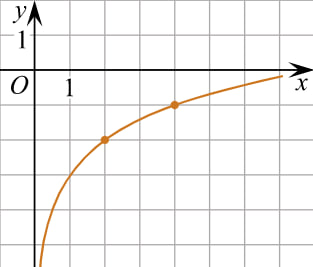
\includegraphics[align=t, width=0.4\linewidth]{\picpath/prob_2_6}
		\end{center}
		\foranswer
		%11
		\item Найдите наименьшее значение функции \( y=10\cos x+17x+3 \) на отрезке \( \left[ 0;\dfrac{3\pi}{2}\right]  \).
		\foranswer
		\egepreambtwo
		\title{Часть 2}
		%12
		\item а) Решите уравнение \( \log_2\sin2x+\log_{\tfrac{1}{2}}\cos x=\dfrac{1}{2} \). \\
		б) Укажите корни этого уравнения, принадлежащие отрезку \( \left[ -\dfrac{5\pi}{2};-\dfrac{\pi}{2} \right]  \).
		\newpage
		\hphantom{Часть 1}
		%13
		\item В основании прямой призмы \( ABCDA_1B_1C_1D_1 \) лежит квадрат \( ABCD \) со стороной \( 2 \), а высота призмы равна \( 1 \). Точка \( E \) лежит на диагонали \( BD_1 \), причём \( BE=1 \).\\
		а)  Постройте сечение призмы плоскостью \( A_1C_1E \).\\		
		б)  Найдите угол между плоскостью сечения и плоскостью \( ABC \).
		%14
		\item Решите неравенство: \( 5\cdot2^{2x+1}-21\cdot2^{x-1}\le0 \)
		%15
		\item Светлана Михайловна взяла кредит в банке на \( 4 \) года на сумму \( 4\: 420\: 000 \) рублей. Условия возврата кредита таковы: в конце каждого года банк увеличивает текущую сумму долга на \( 10\% \). Светлана Михайловна хочет выплатить весь долг двумя равными платежами --- в конце второго и четвертого годов. При этом платежи в каждом случае выплачиваются после начисления процентов. Сколько рублей составит каждый из этих платежей?
		%16
		\item В остроугольном треугольнике \( KMN \) проведены высоты \( KB \) и \( NA \).\\
		а)  Докажите, что угол \( ABK \) равен углу \( ANK \).	\\
		б)  Найдите радиус окружности, описанной около треугольника \( ABM \), если известно, что \( KN=8\sqrt{2} \) и \( \angle KMN=45\degree \).
		%17
		\item Найдите все значения \( a \), для каждого из которых уравнение \[ \log_{1-x}(a-x+2)=2 \] имеет хотя бы один корень, принадлежащий промежутку \( [-1;-1) \).
		%18
		\item Целые числа от \( 1 \) до \( n \) записаны в строчку. Под ними записаны те же числа в другом порядке. Может ли случиться так, что сумма каждого числа и записанного под ним есть точный квадрат.\\
		а)  при \( n=9 \),\\		
		б)  при \( n=11 \),\\		
		в)  при \( n=1996 \).
	\end{listofex}
\end{training}
%END_FOLD